\documentclass{article}
\usepackage[utf8]{inputenc}
\usepackage[spanish]{babel}
\usepackage{amsmath}
\usepackage{amssymb}
\usepackage{amsfonts}
\usepackage{hyperref}
\usepackage{textcomp}
\usepackage{graphicx}
\usepackage{pgfplots}
\usepackage{geometry}
\usepackage{tikz}
\hypersetup{
    colorlinks=true,
    linkcolor=black,
    citecolor=green,
    filecolor=magenta,      
    urlcolor=cyan,
}
\geometry{
  top=3cm,            % Margen superior
  bottom=3cm,         % Margen inferior
  left=3cm,           % Margen izquierdo
  right=3cm           % Margen derecho
}

\title{Estadística 1}
\author{Jorge Miguel Alvarado Reyes}
\date{16 Agosto 2023}

\setlength{\parindent}{0pt}
\begin{document}

\begin{titlepage}
    \begin{center}
        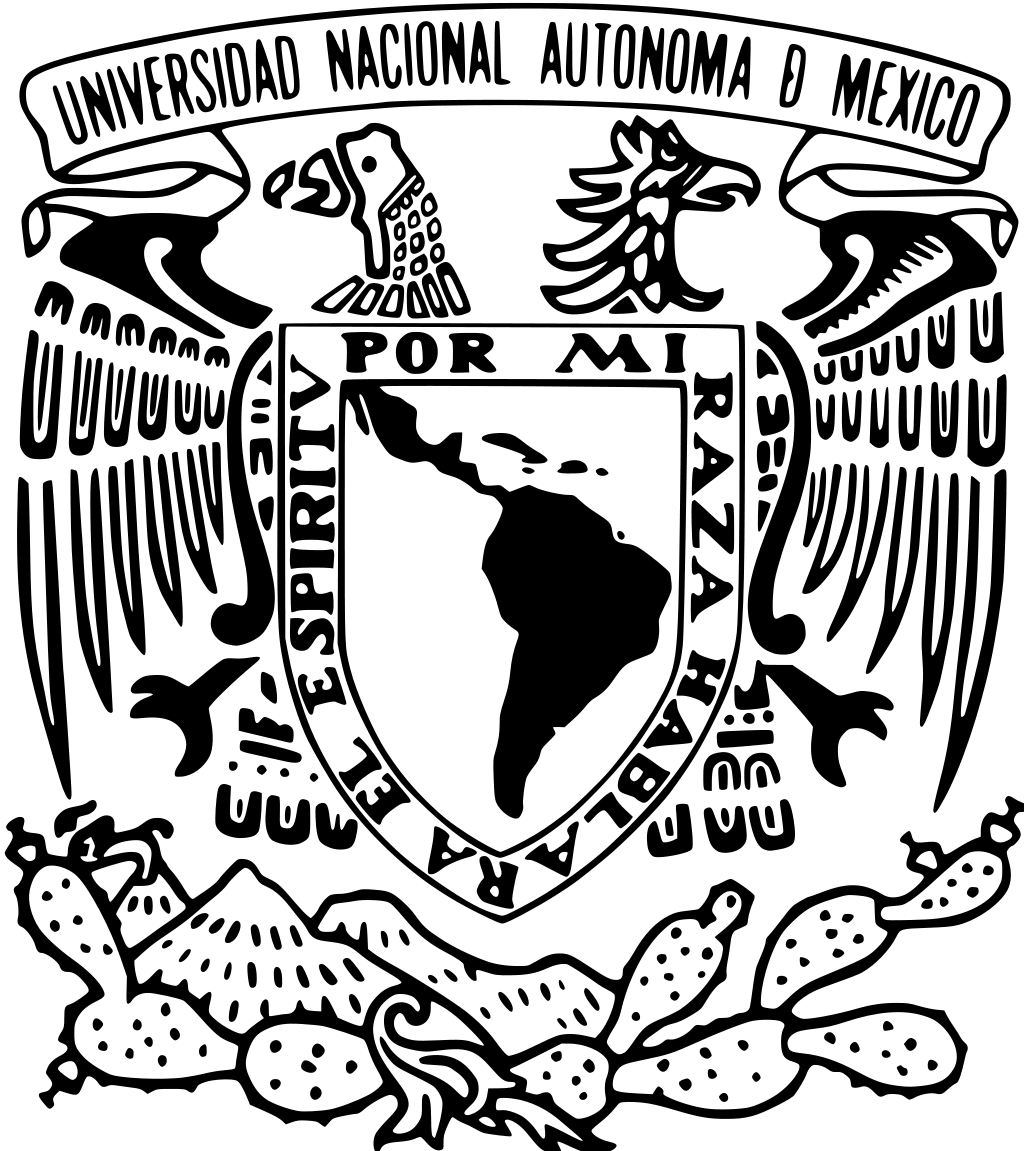
\includegraphics[width=0.2\textwidth]{../../unam.png}
        \vspace*{.5cm}

        \LARGE
        \textbf{Universidad Nacional Autónoma de México}

        \vspace{0.5cm}
        \LARGE
        Facultad de Estudios Superiores Acatlán

        \vspace{2cm}

        \textbf{Apuntes} \\
        Procesos Estocasticos

        \vfill

        \vspace{1cm}

        \textbf{\large Autor:} \\
        Jorge Miguel Alvarado Reyes \\
        \vspace{.5cm}
        \normalsize \today

    \end{center}
\end{titlepage}
\newpage

\tableofcontents

\newpage

\section{Elementos de procesos estocasticos}

\subsection{Definición de procesos estocasticos}

\subsubsection{Ejercicio 1}

Sea \(X_t\) el resultado de la suma sucesiva (acumulada) del lanzamiento de dos dados con solo tres caras. Se realizan 2 lanzamientos.

\begin{enumerate}
    \item Defina \(S\) y \(T\)
    \item Calcule las probabilidades asociadas a cada valor de \(X_1\) y \(X_2\)
\end{enumerate}

\textbf{Nota}

$S$ es el conjunto de todos los estados posibles (Conjunto de estados)
$T$

\subsubsection{Solucion ejercicio 1}

\textbf{Indice 1}
\begin{itemize}
    \item \(S = \{2,3,4,5,6\}\)
    \item \(T = \{1,2\}\)
\end{itemize}

\textbf{Indice 2}

\begin{tabular}{c|c}
    suma de dos lan zamientos & Resultado \\
    \hline
    1+1                       & 2         \\
    1+2                       & 3         \\
    1+3                       & 4         \\
    2+1                       & 3         \\
    2+2                       & 4         \\
    2+3                       & 5         \\
    3+1                       & 4         \\
    3+2                       & 5         \\
    3+3                       & 6         \\
\end{tabular}

\begin{itemize}
    \item $\mathbb{P}(X_t = 2) = 1/9$
    \item $\mathbb{P}(X_t = 3) = 2/9$
    \item $\mathbb{P}(X_t = 4) = 3/9$
    \item $\mathbb{P}(X_t = 5) = 2/9$
    \item $\mathbb{P}(X_t = 6) = 1/9$
\end{itemize}

\newpage

\subsection{Clasificación de procesos estocasticos}

\subsubsection{Ejercicio 2}

Indique la clasificación de cada proceso estocástico, considerándolo de acuerdo a la naturaleza de su conjunto de estados y conjunto paramétrico. Indique los valores de \( s \) y \( t \).

\begin{enumerate}
    \item Es el proceso estocástico que contabiliza la cantidad de lluvia que cae en la ciudad de México cada día.
          \[S = \{x \in \mathbb{R} : x \geq \mathbb{0}\}\]
          \[T = \{1,2,3,\dots\} \text{Cada los dias}\]
    \item Es el proceso estocástico que indica la cantidad de impresoras descompuestas en cada departamento de la FES Acatlán.
          \[S = \{0,1,2,3,\dots\} \]
          \[T = \{1,2,3\} \text{Cada departamento de la FES}\]
    \item Es el proceso estocástico que calcula el porcentaje de enfermos de dengue por colonia en Pachuca, Hidalgo.
          \[S = \{x : x \in [0, 100]\} \]
          \[T = \{1,2,3,\dots,N\} \text{N es el numero de colonias}\]
    \item Es el proceso estocástico que mide el tiempo que tarda en caer la n-ésima pelota lanzada desde el techo de una casa.
          \[S = \{x \in \mathbb{R} : x > 0\}\]
          \[ T = \{1,2,3,\dots\} \text{ correspondiente a cada n-ésima pelota lanzada} \]
    \item Es el proceso estocástico que mide el tiempo de clase diaria que imparte un profesor.
          \[ S = \{x \in \mathbb{R} : x \geq 0\} \]
          \[ T = \{1,2,3,\dots\} \text{ representando cada día de clase} \]
    \item Es el proceso estocástico que mide la cantidad de agua que existe en una cisterna en un instante específico.
          \[ S = \{x \in \mathbb{R} : x \geq 0\} \]
          \[ T = \{t \in \mathbb{R} : t \geq 0\} \text{ representando el tiempo continuo} \]
    \item Es el proceso estocástico que mide el promedio de calificaciones de un grupo de alumnos durante cada semestre, en una carrera que dura 10 semestres.
          \[ S = \{x \in [0, 100]\} \]
          \[ T = \{1,2,3,\dots,10\} \text{ cada semestre de la carrera} \]
    \item Es el proceso estocástico que indica la posición de un elevador de 5 pisos en un instante de tiempo definido.
          \[ S = \{1,2,3,4,5\} \]
          \[ T = \mathbb{R}^+ \text{ tiempo continuo} \]
    \item Es el proceso estocástico que determina el marcador de un partido de tenis, durante 5 sets.
          \[ S = \text{Conjunto de posibles marcadores en tenis} \]
          \[ T = \{1,2,3,4,5\} \text{ correspondiente a cada set del partido} \]
    \item Es el proceso estocástico que mide el porcentaje de llenado individual de 40 botellas en un período de 10 segundos.
          \[ S = \{x \in [0, 100]\} \]
          \[ T = \{t \in \mathbb{R} : 0 \leq t \leq 10\} \]
\end{enumerate}

\subsection{Ejemplos de procesos estocasticos}

\subsubsection{Ejercicio 3 - Tarea 1}

En cada ejercicio determine \( S \), \( T \) y si es posible, las probabilidades de transición (como fórmula, tabla o gráfica)

\begin{enumerate}
    \item Un alumno realiza apuestas de \$10 con una probabilidad ``\( p \)'' de ganar, una probabilidad ``\( q \)'' de perder y una probabilidad ``\( r \)'' de quedarse igual. Inicia el juego con un capital de \$100. Se retira del juego si pierde todo su capital o si lo duplica. Sea \( X_t \) el capital del alumno después de la t-ésima apuesta.
          \[ S = \{0, 10, 20, \dots, 200\} \]
          \[ T = \{1,2,3,\dots\} \text{Numero de apuestas}\]
          \begin{center}
              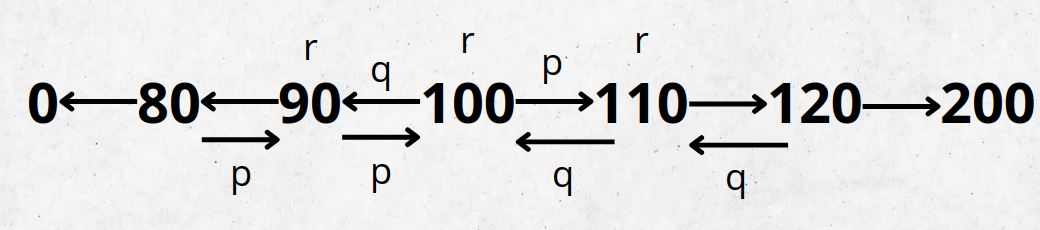
\includegraphics[width=0.6\linewidth]{./imagenes/image.png}
          \end{center}
    \item Suponer que al final de cada año escolar un estudiante tiene que repetir el año o pasar al curso siguiente. Considere que se requiere un mínimo de 3 años para completar el nivel académico.
          \[ S = \{1,2,3\} \text{Cada uno de los semestres que va a cursar}\]
          \[T = \{1,2,3,\dots\}\text{evaluacion al final de cada año que determina si el alumno pasa o no}\]
          \begin{center}
              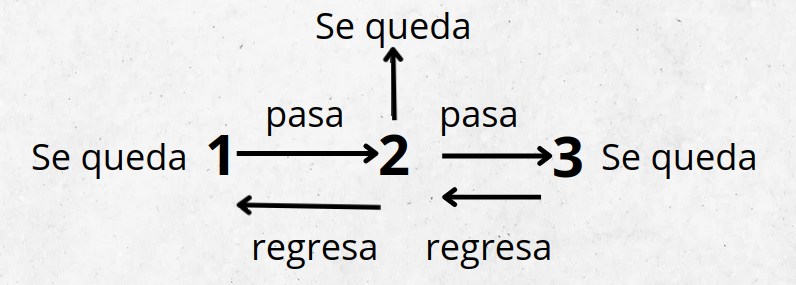
\includegraphics[width=0.6\linewidth]{./imagenes/image2.png}
          \end{center}
    \item Suponer que se lleva un control del comportamiento del dólar en cada día, considerando que baja, sube o se mantiene.
          \[S = {\text{Baja}, \text{Sube}, \text{Se mantiene}}\]
          \[T = {1,2,3,\dots} \text{Dias en los que s ehace la medicion}\]
    \item Constrúyase un proceso para estudiar el escrutinio de los votos de una justa electoral entre sólo 2 candidatos.
          \[T = \{1,2\dots, n\} \text{Numero de votos a contar}\]
    \item Una fábrica tiene 2 máquinas, pero en cualquier día dado no se usa más que una. Esta máquina tiene una probabilidad constante \( p \) de sufrir una avería, y si así sucede, la avería ocurre la final del trabajo del día. Se emplea un solo hombre para repararla. A este hombre le toma 2 días reparar la máquina y sólo trabaja en una máquina a la vez. Considere que \( X_t \) es el proceso estocástico que registra al final del día \( t \), el número de días que serán necesarios para que ambas máquinas trabajen.
          \[T = \{1,2,3,\dots\} \text{Dias en los que se eobserva la disponibilidad}\]
\end{enumerate}

\subsection{Conceptos básicos de procesos estocasticos}

\subsubsection{Ejercicio 4 - Ejercicios de clase, procesos de bernoulli y caminata aleatoria}

\subsection*{Problema 1}
Demuestre que para un $N_n$ definido en un proceso de Bernoulli, la varianza, $\text{Var}(N_n)$, es igual a $npq$
Sea \( X \) el número de éxitos, entonces:
\[ E(N_n) = np \]

Para cualquier \( X_i \):
\[ P(X_i = 1) = p \text{ Exito}\]
\[ P(X_i = 0) = 1 - p = q \text{ Fracaso}\]

Entonces la esperanza de \( X \) es:
\[ E(N_n) = E(X_1) + E(X_2) + \ldots + E(X_n) \]

Para cualquier \( X_i \):
\[ E(X_i) = 0 \cdot q + 1 \cdot p = p \]

Entonces:
\[ E(N_n) = p + p + p \text{ Asi n veces}\]
\[ E(N_n) = np\]

ahora debemos encontrar $E(N_n^2)$

\[E(N_n^2) = \sum_{k=0}^{n} k^2 \cdot P(N_n = k)\]

\[P(N_n = k) = \binom{n}{k} p^k q^{n-k}\]

entonces

\[E(N_n^2) = \sum_{k=0}^{n} \binom{n}{k} p^k q^{n-k}\]

\[E(N_n^2) = npq + (np)^2\]

Entonces la varianza es

\[Var(N_n) = E(N_n^2) - E(N_n)^2\]

\[Var(N_n) = npq + (np)^2 - (np)^2\]

\[Var(N_n) = npq\]

\subsection*{Problema 2}

Demuestre que la funcion generatriz de momentos de la caminata aleatoria es $M(t) = (pe^t + qe^{-t}) * n$. Recuerda que la funcion generatriz de momentos es: $m(t) = E(e^{tx})$


\subsubsection*{Paso 1: Definición de la Función Generatriz de Momentos}
La función generatriz de momentos $m(t)$ de una variable aleatoria $X$ se define como:
\[ m(t) = E[e^{tX}] \]

\subsubsection*{Paso 2: Aplicación a la Caminata Aleatoria}
Para un solo paso $X_i$ de la caminata, donde $X_i = +1$ con probabilidad $p$ y $X_i = -1$ con probabilidad $q$, la función generatriz de momentos es:
\[ m_i(t) = E[e^{tX_i}] = pe^{t(+1)} + qe^{t(-1)} = pe^t + qe^{-t} \]

\subsubsection*{Paso 3: Función Generatriz de Momentos para $n$ Pasos}
Considerando que la caminata aleatoria está compuesta por $n$ pasos independientes y que la función generatriz de momentos para la suma de variables aleatorias independientes es el producto de sus funciones generatriz de momentos individuales, la función generatriz de momentos para la caminata aleatoria completa, $M(t)$, es:
\[ M(t) = (m_i(t))^n = (pe^t + qe^{-t})^n \]


\subsection*{Problema 3}

Demuestre que para $n,k \in \{1,2,3,\dots\}$

\[P\{N_{n+1} = k\} = p * P\{N_n = k-1\} + q * P\{N_n = k\}\]

donde $N_n$ es el número de éxitos en $n$ ensayos de Bernoulli, $p$ es la probabilidad de éxito, y $q = 1 - p$ es la probabilidad de fracaso.

Utilizando la ley de probabilidad total:
\[ P\{N_{n+1} = k\} = P\{N_{n+1} = k | N_n = k-1\} \cdot P\{N_n = k-1\} + P\{N_{n+1} = k | N_n = k\} \cdot P\{N_n = k\} \]

En un ensayo solo puede ocurrir un éxito o un fracaso:
\[ P\{N_{n+1} = k | N_n = k-1\} = p \]
\[ P\{N_{n+1} = k | N_n = k\} = q \]

La fórmula se reduce a:
\[ P\{N_{n+1} = k\} = p \cdot P\{N_n = k-1\} + q \cdot P\{N_n = k\} \]

\newpage

\subsubsection{Ejercicio 5 - Ejercicios caminata aleatoria y distribucion de probabilidad}

\subsection*{Problema 1}

Demuestre la formula de probabilidades de transicion de una caminata alaeatoria simple usando ahora los pasos que se dan a la izquierda

\subsection*{Problema 2}

Para una caminata aleatoria simple \(X_n\) sobre los enteros, demuestre que:
\[ P(X_{n+1} = x) = pP(X_n = x - 1) + qP(X_n = x + 1) \]

Sugerencia: Sustituya los parámetros de las probabilidades en la fórmula de probabilidades de transición de una caminata aleatoria y con álgebra verifique la igualdad.

\subsection*{Problema 3}

Una partícula realiza una caminata aleatoria simétrica sobre los enteros empezando en 0. Encuentre la probabilidad de que la partícula no se encuentre nuevamente en el origen en el sexto paso.

\subsubsection{Ejercicio 6 - Practica 2: Caminata aleatoria}

\subsection*{Problema 1}

Considere que existe una partícula que realiza una caminata aleatoria sobre los números enteros, iniciando en 3. La probabilidad de dar un paso a la derecha es de \( \frac{2}{3} \). Encuentre la probabilidad de que la partícula se encuentre:

\begin{enumerate}
    \item[a)] En la posición 8 en 10 pasos.
    \item[b)] Regrese a la posición 3 en 6 pasos.
\end{enumerate}

\subsubsection*{Punto a}

La probabilidad de que la partícula se encuentre en la posición 8 después de 10 pasos es:
\[
    P\{X_{10} = 8 | X_0 = 3\} = \binom{10}{\frac{10 + 8 - 3}{2}} \left(\frac{2}{3}\right)^{\frac{10 + 8 - 3}{2}} \left(\frac{1}{3}\right)^{\frac{10 - 8 + 3}{2}},
\]
dado que \( \frac{10 + 8 - 3}{2} \) no es un número entero, la probabilidad es 0. esto se debe a que no se puede llegar a una posicion par dando un numero par de pasos desde una posicion inicial impar

\[
    P\{X_{10} = 8 | X_0 = 3\} = 0
\]

\subsubsection*{Punto b}

La probabilidad de que la partícula regrese a la posición 3 en 6 pasos es:
\[
    P\{X_6 = 3 | X_0 = 3\} = \binom{6}{\frac{6 + 3 - 3}{2}} \left(\frac{2}{3}\right)^{\frac{6 + 3 - 3}{2}} \left(\frac{1}{3}\right)^{\frac{6 - 3 + 3}{2}},
\]
aplicando los valores obtenemos que la probabilidad es aproximadamente 0.2195 o 21.95\%.

\subsection*{Problema 2}

Considere una partícula que realiza una caminata aleatoria simple simétrica sobre los enteros. Encuentre la probabilidad de que la partícula se encuentre:

\begin{enumerate}
    \item[a)] En la posición 5 en 9 pasos.
    \item[b)] En la posicion 3 o 7 en 10 pasos
    \item[c)] En la posicion 2 en 7 pasos
\end{enumerate}

\subsubsection*{Punto a}


La probabilidad de que la partícula se encuentre en la posición 5 después de 9 pasos, comenzando desde una posición inicial \(X_0\), es:
\[
    P\{X_9 = 5 | X_0 = X_0\} = \binom{9}{7} \left(\frac{1}{2}\right)^{7} \left(\frac{1}{2}\right)^{2},
\]

\[
    P\{X_9 = 5 | X_0 = X_0\} = \binom{9}{7} \left(\frac{1}{2}\right)^{9},
\]

\[
    P\{X_9 = 5 | X_0 = X_0\} = 0.0703125,
\]
lo que representa una probabilidad del 7.03125\%.

\subsubsection*{Punto b}

\[
    P\{X_{13} = 3 | X_0 = 0\} = \binom{13}{8} \left(\frac{1}{2}\right)^{8} \left(\frac{1}{2}\right)^{5} = 0.1571,
\]

\[
    P\{X_{13} =7 | X_0 = 0\} = \binom{13}{10} \left(\frac{1}{2}\right)^{10} \left(\frac{1}{2}\right)^{3} = 0.0349,
\]

\[
    P\{X_{13} = 3 | X_0 = 0\} \cup  P\{X_{13} =7 | X_0 = 0\} = 0.1571 + 0.0349 = 0.1920
\]

\subsubsection*{Punto c}

No es posible llegar a una posicion par dando un numero impar de pasos

\subsection*{Problema 3}

Considere una persona que bajo los efectos del alcohol da pasos hacia
delante con probabilidad de $0.57$ y hacia atrás con probabilidad
complementaria, sobre una calle que puede referenciarse con los números
enteros. Él sale de la cantina que se encuentra en la posición $-3$. Su casa se
encuentra en la posición $4$. La casa de su mejor amigo en la posición $2$ y un
Oxxo en el origen. Considere la probabilidad de que el borracho, saliendo de
la cantina:

\begin{itemize}
    \item[a)] se encuentre en su casa después de $5$ pasos.
    \item[b)] se encuentre en su casa después de $13$ pasos.
    \item[c)] llegue al Oxxo para comprar más alcohol después de $5$ pasos.
    \item[d)] no ``caiga en la casa de su mejor amigo'' en $9$ pasos.
\end{itemize}

\subsubsection*{Punto a}

\[
    P\{X_{5} = 4 | X_0 = -3\} = \binom{5}{\frac{5+4+3}{2}} \left(0.57\right)^{\frac{5+4+3}{2}} \left(0.43\right)^{\frac{5-4-3}{2}}
\]

El numero de pasos para llegar de \(-3\) a \(4\) es de minimo 7 por lo tanto con 5 pasos no se puede llegar

\subsubsection*{Punto b}

\begin{align*}
    P\{X_{13} = 4 \mid X_0 = -3\} & = \binom{13}{\frac{13+4-(-3)}{2}} \left(0.57\right)^{\frac{13 + 4 - (-3)}{2}} \left(0.43\right)^{\frac{13 - 4 + (-3)}{2}} \\
                                  & = \binom{13}{\frac{14}{2}} \left(0.57\right)^{\frac{14}{2}} \left(0.43\right)^{\frac{6}{2}}                               \\
                                  & = \binom{13}{7} \left(0.57\right)^{7} \left(0.43\right)^{3}                                                               \\
                                  & = 0.2120
\end{align*}

\subsubsection*{Punto c}

\begin{align*}
    P\{X_{5} = 0 \mid X_0 = -3\} & = \binom{5}{\frac{5 + 0-(-3)}{2}} \left(0.57\right)^{\frac{5 + 0 - (-3)}{2}} \left(0.43\right)^{\frac{5 - 0 + (-3)}{2}} \\
                                 & = \binom{5}{\frac{8}{2}} \left(0.57\right)^{\frac{8}{2}} \left(0.43\right)^{\frac{2}{2}}                                \\
                                 & = \binom{5}{4} \left(0.57\right)^{4} \left(0.43\right)                                                                  \\
                                 & = 0.2269
\end{align*}

\subsubsection*{Punto d}

\begin{align*}
    P\{X_{9} = 2 \mid X_0 = -3\} & = \binom{9}{\frac{9 + 2 -(-3)}{2}} \left(0.57\right)^{\frac{9 + 2 - (-3)}{2}} \left(0.43\right)^{\frac{9 - 2 + (-3)}{2}} \\
                                 & = \binom{5}{\frac{14}{2}} \left(0.57\right)^{\frac{14}{2}} \left(0.43\right)^{\frac{4}{2}}                               \\
                                 & = \binom{5}{7} \left(0.57\right)^{4} \left(0.43\right)^{2}                                                               \\
                                 & = 0.1302
\end{align*}

La probabilidad de que no caiga es $1-0.1302 = 0.8698$

\section{Cadena de markov}

\subsection{Problema 1}

Considere el modelo del valor de una acción. Al final de un día dado se registra el precio. Si la acción subió la probabilidad de que suba mañana es de 0.7. Si la acción bajó, la probabilidad de que suba mañana es de sólo 0.5. (Por simplicidad, cuando una acción permanezca con el mismo valor, se considerará un aumento)

El \textbf{espacio de estados} \( S \) es definido como:

\[ S = \{ \text{Sube}, \text{Baja} \} \]

Donde:
\begin{itemize}
    \item "Sube" indica que el precio de la acción sube o permanece igual (considerado como aumento).
    \item "Baja" indica que el precio de la acción baja.
\end{itemize}

% Matriz de Transición
La \textbf{matriz de transición} \( P \) representa las probabilidades de pasar de un estado a otro. Para este modelo, la matriz es:
\[ P = \begin{pmatrix} 0.7 & 0.3 \\ 0.5 & 0.5 \end{pmatrix} \]

Donde:
\begin{itemize}
    \item La primera fila \( \begin{pmatrix} 0.7 & 0.3 \end{pmatrix} \) representa las probabilidades de transición desde el estado "Sube": Si hoy el precio subió (o se mantuvo igual), la probabilidad de que suba mañana es de 0.7 y la de que baje es de 0.3.
    \item La segunda fila \( \begin{pmatrix} 0.5 & 0.5 \end{pmatrix} \) representa las probabilidades de transición desde el estado "Baja": Si hoy el precio bajó, la probabilidad de que suba mañana es de 0.5 y la de que baje es también de 0.5.
\end{itemize}

\subsection{Problema 2}

Suponga ahora que el modelo de mercado de acciones se cambia de manera que el hecho de que una acción suba o no mañana, depende de si subió o no hoy y ayer. En particular, si la acción subió los dos días, ayer y hoy, la probabilidad de que suba mañana es de 0.9. Si la acción subió hoy, pero ayer bajó, la probabilidad de que mañana suba es de 0.6. Si la acción bajó hoy pero ayer subió la probabilidad de que mañana suba es de 0.5. Si bajó durante estos 2 días, la probabilidad de que mañana suba es de 0.3.

Considere solo 4 estados, SUBIÓ-SUBIÓ, SUBIÓ-BAJÓ, BAJÓ-SUBIÓ, BAJÓ-BAJÓ.

\[S={SUBIO-SUBIO,SUBIO-BAJO,BAJO-SUBIO,BAJO-BAJO}\]

\[
    P = \begin{bmatrix}
        0.9 & 0.1 & 0   & 0   \\
        0   & 0   & 0.6 & 0.4 \\
        0.5 & 0.5 & 0   & 0   \\
        0   & 0   & 0.3 & 0.7 \\
    \end{bmatrix}
\]

\subsection{Problema 3}

La compañía Colgate ha estado promoviendo un nuevo tipo de detergente. El resultado de dicha promoción es que el 75\% de las personas que usan el detergente durante un período de un mes continúan utilizándolo. De las personas que usan otro detergente durante un período de un mes, un 45\% cambia al detergente de Colgate al mes siguiente.


Definimos el \textbf{espacio de estados} \( S \) como:
\[ S = \{ \text{Colgate}, \text{Otro} \} \]

La \textbf{matriz de transición} \( P \) es:
\[
    P = \begin{pmatrix}
        0.75 & 0.25 \\
        0.45 & 0.55 \\
    \end{pmatrix}
\]

\section{Practica 4}

\subsection*{Problema 1}

Suponga que hay 3 periódicos dominicales: Excelsior, El Universal y La Prensa.
Y suponga además que cada persona cada domingo compra solo uno de ellos. Supongase los siguiente porcentajes de cambio de periódico al paso de los años

\begin{itemize}
    \item[a)] 80\% siguen comprando el mismo periódico de un año para otro
    \item[b)] De los lectores de Excelsior, el 15\% cambia a El Universal
    \item[c)] De los lectores de El Universal el 10\% cambia a La Prensa
    \item[d)] De los lectores de La Prensa, el 8\% cambian a Excelsior
\end{itemize}

Escriba la matriz de transición de un y de 3 pasos. Determine las probabilidades de las siguientes sucesiones suponiendo que el primero de los periódicos de las series tiene una probabilidad de 1:

\begin{enumerate}
    \item Excelsior-El Universal-La Prensa
    \item La Prensa-El Universal-Excelsior
    \item El Universal-Excelsior-La Prensa
\end{enumerate}

\subsubsection*{Solucion}

\begin{itemize}
    \item $P(E \rightarrow E) = 80\%$,
    \item $P(E \rightarrow U) = 15\%$,
    \item $P(E \rightarrow P) = 5\%$, dado que $100\% - 80\% - 15\% = 5\%$,
    \item $P(U \rightarrow U) = 80\%$,
    \item $P(U \rightarrow P) = 10\%$,
    \item $P(U \rightarrow E) = 10\%$, dado que $100\% - 80\% - 10\% = 10\%$,
    \item $P(P \rightarrow P) = 80\%$,
    \item $P(P \rightarrow E) = 8\%$,
    \item $P(P \rightarrow U) = 12\%$, dado que $100\% - 80\% - 8\% = 12\%$.
\end{itemize}

Esto nos da la matriz de transición \(P\) para 1 paso (en forma de porcentaje):

\[ P = \begin{bmatrix} 0.8 & 0.15 & 0.05 \\ 0.1 & 0.8 & 0.1 \\ 0.08 & 0.12 & 0.8 \end{bmatrix} \]

La matriz de transición de 3 pasos, obtenida elevando la matriz de 1 paso al cubo, es:

\[ P^3 = \begin{bmatrix} 0.5594 & 0.30705 & 0.13355 \\ 0.2143 & 0.5786 & 0.2071 \\ 0.18488 & 0.26292 & 0.5522 \end{bmatrix} \]

\begin{enumerate}
    \item Excelsior-El Universal-La Prensa, $P(E \rightarrow U) * P(U \rightarrow P) = 1.5\%$
    \item La Prensa-El Universal-Excelsior $P(P \rightarrow U) * P(U \rightarrow E) = 1.2\%$
    \item El Universal-Excelsior-La Prensa $P(U \rightarrow E) * P(E \rightarrow P) = 0.05\%$
\end{enumerate}

\subsection*{Problema 2}

Tres supermercados locales x, y, z compiten por los precios; una investigación descubre que cada mes el cambio de supermercados se da en las siguientes proporciones:
\begin{itemize}
    \item[a)] X conserva el 80\% de sus clientes y gana 10\% de los de Y y 2\% de los de Z
    \item[b)] Y conserva el 70\% de sus clientes, gana 14\% de los de X y 8\% de los de Z
    \item[c)] Z conserva el 90\% de sus clientes, gana 6\% de X y 20\% de Y
\end{itemize}

Obtener la matriz de transición para el porcentaje de cambios por mes. ¿Cuál es porcentaje de clientes que tendrá cada supermercado en septiembre, suponiendo que la matriz calculada para el mes de junio?

\subsubsection*{Solucion}

\begin{table}[ht]
    \centering
    \begin{tabular}{|l|c c c|}
        \hline
          & x    & y    & z    \\ \hline
        x & 0.80 & 0.14 & 0.06 \\
        y & 0.10 & 0.70 & 0.20 \\
        z & 0.02 & 0.08 & 0.90 \\
        \hline
    \end{tabular}
\end{table}

Donde la columna es la marca que obtiene el porcentaje del renglon, ejemplo la columna x en su renglon y significa que x gana el $10\%$ de sus clientes de y

\newpage

\subsection*{Problema 3}

El departamento de estudios de mercado de una fábrica estima que el 20\% de la gente que compra un producto un mes, no lo comprará el mes siguiente. Además el 30\% de quienes no lo compren un mes lo adquirirá al mes siguiente. En una población de 1000 individuos, 100 compraron el producto el primer mes. Construya la matriz de transición e indique ¿cuántos lo comprarán el mes próximo? ¿Y dentro de dos meses?

\subsubsection*{Solucion}

Primero definimos la matriz de transición \(T\) y el vector de estado inicial \(\vec{v}_0\):

\[
    T = \begin{pmatrix}
        0.8 & 0.2 \\
        0.3 & 0.7
    \end{pmatrix},
    \quad
    \vec{v}_0 = \begin{pmatrix}
        100 \\
        900
    \end{pmatrix}
\]

Para calcular cuántas personas comprarán el producto el mes próximo (\(\vec{v}_1\)), multiplicamos la matriz de transición \(T\) por el vector de estado inicial \(\vec{v}_0\):

\[
    \vec{v}_1 = T \cdot \vec{v}_0 = \begin{pmatrix}
        0.8 & 0.2 \\
        0.3 & 0.7
    \end{pmatrix}
    \cdot
    \begin{pmatrix}
        100 \\
        900
    \end{pmatrix}
    =
    \begin{pmatrix}
        260 \\
        740
    \end{pmatrix}
\]

Esto significa que 260 personas comprarán el producto el mes próximo.

Para calcular cuántas personas lo comprarán dentro de dos meses (\(\vec{v}_2\)), multiplicamos la matriz de transición \(T\) por el vector de estado después de 1 mes \(\vec{v}_1\):

\[
    \vec{v}_2 = T \cdot \vec{v}_1 = \begin{pmatrix}
        0.8 & 0.2 \\
        0.3 & 0.7
    \end{pmatrix}
    \cdot
    \begin{pmatrix}
        260 \\
        740
    \end{pmatrix}
    =
    \begin{pmatrix}
        340 \\
        660
    \end{pmatrix}
\]

Lo que indica que 340 personas comprarán el producto dentro de dos meses.


\subsection*{Problema 4}

En una población de 10000 habitantes, 5000 no fuman, 2500 fuman uno o menos de un paquete diario y 2500 fuman más de un paquete diario. En un mes hay un 5\% de probabilidad de que un no fumador comience a fumar un paquete diario o menos, y un 2\% de que un no fumador pase a fumar más de un paquete diario. Para los que fuman un paquete o menos, hay un 10\% de probabilidad de que dejen el tabaco y un 10\% de que pasen a fumar más de un paquete diario. Entre los que fuman más de un paquete hay un 5\% de probabilidad de que dejen el tabaco y un 10\% de que pasen a fumar un paquete o menos. Obtenga la matriz de transición e indique ¿cuántos individuos habrá de cada clase el próximo mes?

Primero, definimos la matriz de transición \(T\) y el vector de estado inicial \(\vec{v}_0\):

\[
    T = \begin{pmatrix}
        0.93 & 0.05 & 0.02 \\
        0.10 & 0.80 & 0.10 \\
        0.05 & 0.10 & 0.85
    \end{pmatrix},
    \quad
    \vec{v}_0 = \begin{pmatrix}
        5000 \\
        2500 \\
        2500
    \end{pmatrix}
\]

Para encontrar cuántos individuos habrá de cada clase el próximo mes (\(\vec{v}_1\)), multiplicamos la matriz de transición \(T\) por el vector de estado inicial \(\vec{v}_0\):

\[
    \vec{v}_1 = T \cdot \vec{v}_0 = \begin{pmatrix}
        0.93 & 0.05 & 0.02 \\
        0.10 & 0.80 & 0.10 \\
        0.05 & 0.10 & 0.85
    \end{pmatrix}
    \cdot
    \begin{pmatrix}
        5000 \\
        2500 \\
        2500
    \end{pmatrix}
    =
    \begin{pmatrix}
        4825 \\
        2750 \\
        2625
    \end{pmatrix}
\]

Esto indica que habrá 4825 individuos que no fuman, 2750 que fuman un paquete o menos al día, y 2625 que fuman más de un paquete al día el próximo mes.


\end{document}